%!TEX root = ../thesis.tex

\chapter{Artefacts in Optimal Extraction} % Main appendix title
\label{appendix:artefacts}

% Table of nods optimally reduced replaced by rectangular extraction and bad pixel replacement.
%!TEX root = ../../thesis.tex
% Table of nods replaced for correction.
\change{Maybe transpose \cref{tab:nod_replacement} to be shorter?}{}
\change{CHANGE \# into the ESO identification number 1b 2a etc}
\begin{table}
    \caption{Identification of all the optimally reduced nod spectra which had artefacts that were replaced by the rectangular extractions, corrected for bad pixels. The numbers represent the position in the nod cycle ABBAABBA.\@The number of the observation for each target is given by \#.}
    \label{tab:nod_replacement}
    \centering
    \begin{tabular}{cccccccc}
        \toprule
      & & \multicolumn{4}{c}{Detector}& \\
         Target  & \#  & 1 & 2 & 3 & 4 & Total \\
        \midrule
        \object{HD 4747}   & 1 & 8 & 5, 8 & 8 & 1, 5, 8 & 7\\
        \object{HD 162020} & 1 & - & 7, 8& - & - & 2\\
        \object{HD 162020} & 2 & - & 2 & - & 8 & 2\\
        \object{HD 167665} & 1 & 2, 4 & 8 & 1, 6 &  4, 5 & 7\\
        \object{HD 167665} & 2 & 2 & 3 & 1 & 8 & 4\\
        \object{HD 167665} & 3 & 6 & 3, 7 & - & 8 & 4\\
        \object{HD 168443} & 1& - & - & - & 7, 8 & 2\\
        \object{HD 168443} & 2 & - & 2, 4 & 6 & 8 & 4\\
        \object{HD 202206} & 1 & - & 6, 7& 1& - & 3\\
        \object{HD 202206} & 2 & 5 & - & 7,8 & - & 3\\
        \object{HD 202206} & 3 & 8 & 3 &  6 & 6 & 4\\
        \object{HD 211847} & 1 & - & 5, 7 & 2 & 4 & 4\\
        \object{HD 211847} & 2 & 2 & 1, 7 & 7 & 8 & 5\\
        \object{HD 30501}  & 1 & 7 & 7 & - & 8 & 3\\
        \object{HD 30501}  & 2 & 7, 8 & 3, 5, 7, 8 & 2, 7 & 2, 3&10 \\
        \object{HD 30501}  & 3 & 4, 8 & 2, 6, 7& 4, 8 & 7& 8\\
        \object{HD 30501}  & 4 & 1, 2, 4 & 3 & 5, 6 & 6 & 7\\
         \midrule
            &&16&27&17&19& 79/544\\
    \bottomrule
    \end{tabular}
\end{table}


%!TEX root = ../../thesis.tex
% Tally nods replaced for correction.
\begin{table}
    \centering
    \caption{Tally of nod cycle positions in which their optimally reduced spectra were affected and were replaced.}
    \begin{tabular}{lccccccccr}
        \toprule
        Order Number & 1 & 2 & 3 & 4 & 5 & 6 & 7 & 8 &Total\\
        Nod Position & A & B & B & A & A & B & B & A & \\
        \midrule
        Tally & 6 & 10 & 6 & 7 & 7 & 9 & 15 & 19 & 79\\
        \bottomrule
    \end{tabular}\label{tab:nod_artefact_tally}
\end{table}

As mentioned in \sref{subsubsec:reductionartefacts} there were artefacts observed from the optimal reduction of the {DRACS} pipeline. A list of all specific nods of each observation and detector that were observed to contain artefacts and were replaced with the method developed are provided in \tref{tab:nod_replacement}.

With 8 nods per observation, and 4 detectors for the 17 observation there are 544 individual nod spectra. \tref{tab:nod_replacement} identifies 79 individual nods that contain artefacts which is 14.5\%. Only 16/68 (23.5\%) detector observations have nods without any artefacts and no single observation has no artefacts in any nod spectra across the 4 detectors.

In \tref{tab:nod_artefact_tally} a tally is provided of the frequency of artefacts occurring within each nod in the nod cycle. There is a higher number of artefacts occurring in the last two nod, indicating that there may be something to do with the length of the observation. \todo{Is this significant??}.
There is also a larger number of artefacts occurring on the second detector. This maybe coincidence as it is easier to identify the artefacts with a low number of spectral lines from the target, or possibly something physical to do with detector 2. This is beyond the scope of this work, \todo{is detector two significant as well?}

In this appendix we also provide more example images of the artefacts observed from the optimal reduction of the {DRACS} pipeline. We have selected one observation and detector for each observed target to show a variety of the artefacts observed.

In each image the top panel contains the 8 nod spectra extracted using the optimal method, including variance weighting. The middle panel contains the rectangular extraction (sum of the aperture), including the bad pixels.

It is clear that the large extracted artefacts occur due to single spikes observed in the rectangular extraction. What is unclear is why it only occurs some of the time.

summary of exmaples::: they show...  almost random big and large spikes but not all.

\todo{THESE need to be properly selected and a caption given, one without any artefacts also?}
\todo{Style needs to be tweaked also}


 \begin{figure}
     \centering
     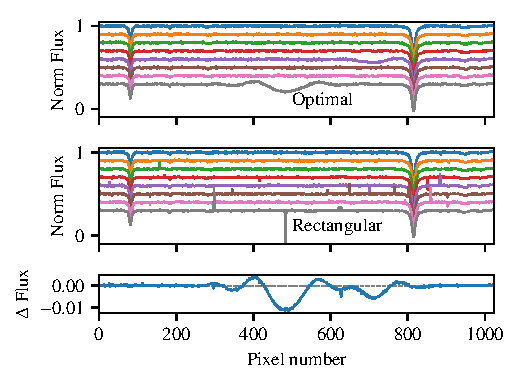
\includegraphics[width=0.9\linewidth]{figures/appendix/bp_plots/extraction_comparision_HD4747-1_chip_2}
     \caption{Artefact example for the second detector of {HD\,4747}.  The top panel contains the 8 normalized nod spectra obtained using optimal extraction. The middle panel shows nod spectra using only rectangular extraction. The bottom panel shows the difference between a combined spectrum using optimal nods only and a combined spectrum in which the identified nods are replaced with their rectangular counterparts as per \sref{subsubsec:reductionartefacts}. A vertical offset is included between each spectra for clarity. The nod spectra are in observation order from top to bottom. In this example there are artefacts in the 5th (purple) and 8th (grey) nod spectra around 700 and 500 pixels respectively.}
     \label{fig:artefact_example1}
 \end{figure}
 \begin{figure}
     \centering
     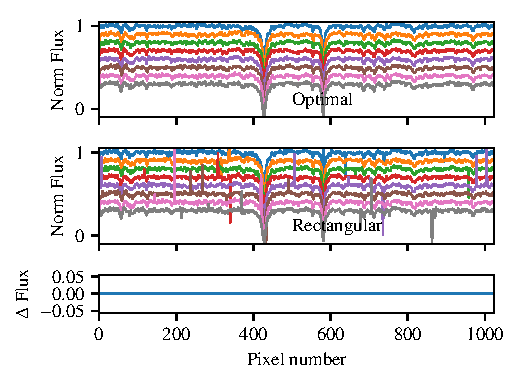
\includegraphics[width=0.7\linewidth]{figures/appendix/bp_plots/extraction_comparision_HD162020-2_chip_1}
     \caption{Same as \fref{fig:artefact_example1} but for the first detector of the second observation of {HD\,162020}. In this example there are several large spikes observed in the rectangular extraction but they do not appear to effect the optimally extracted nods. {\red{} reduce scale of delta flux (to large atm)}.}
     \label{fig:artefact_example2}
 \end{figure}
\todo{change scale on delta flux of {HD\,162020}-2 chip 1 (it is too large atm)}
 \begin{figure}
     \centering
     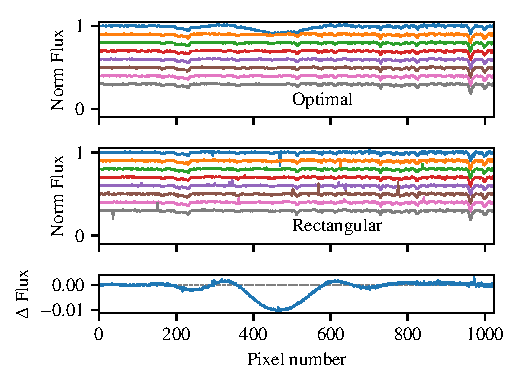
\includegraphics[width=0.7\linewidth]{figures/appendix/bp_plots/extraction_comparision_HD167665-1b_chip_3}
     \caption{Same as \fref{fig:artefact_example1} but for the third detector of the second observation of {HD\,167665}. In this example a small spike in the first spectrum (blue) around pixel 450 causes a extended dip in the optimally extracted nod.}
     \label{fig:artefact_example3}
 \end{figure}
 \begin{figure}
    \centering
    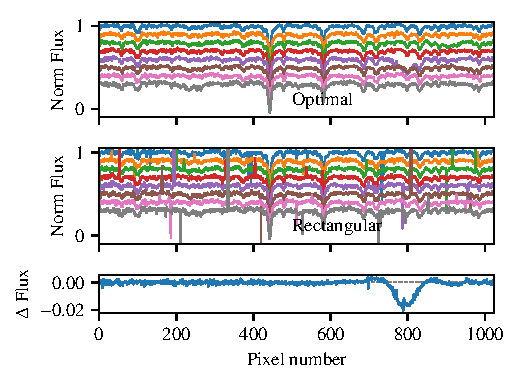
\includegraphics[width=0.7\linewidth]{figures/appendix/bp_plots/extraction_comparision_HD202206-2_chip_1}
    \caption{Same as \fref{fig:artefact_example1} but for the first detector of the second observation of  {HD\,202206}. In this example there are several large spike but only one produces an artefact. This is on the fifth nod (purple) around pixel 800.}
    \label{fig:artefact_example4}
\end{figure}
 \begin{figure}
     \centering
     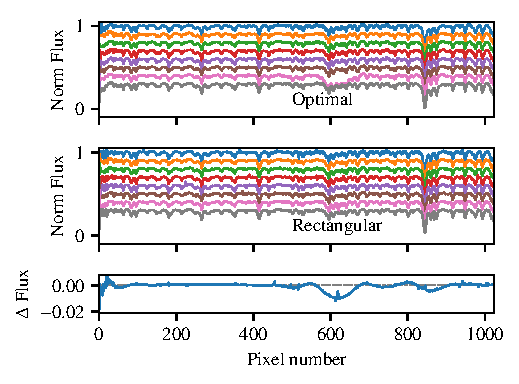
\includegraphics[width=0.7\linewidth]{figures/appendix/bp_plots/extraction_comparision_HD168443-1_chip_4}
     \caption{Same as \fref{fig:artefact_example1} but for the fourth detector of the first observation of {HD\,168443}. In this example a barely visible spike on the seventh nod (pink) causes a deviation in the optimal nod around pixel 610. There is also a second small spike on the eighth  nod (grey) around pixel 850, between two spectral lines.}
     \label{fig:artefact_example5}
 \end{figure}
  \begin{figure}
     \centering
     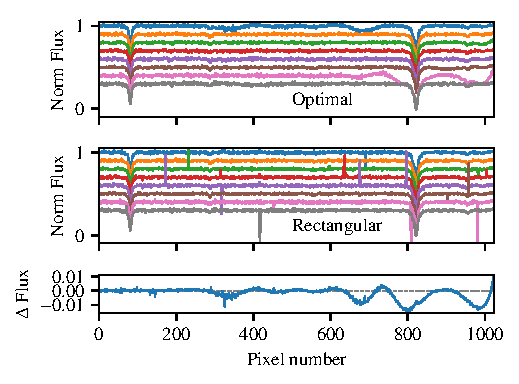
\includegraphics[width=0.7\linewidth]{figures/appendix/bp_plots/extraction_comparision_HD211847-2_chip_2}
     \caption{Same as \fref{fig:artefact_example1} but for the second detector of the second observation of {HD\,211847}. In this example two large spikes around 800 and 1000 in the seventh nod (pink) create large deviations in the optimally reduced spectra. A spike in the first nod (blue) around pixel 700 also causes a bump. There is also some extra noise in the first nod around pixel 350.}
     \label{fig:artefact_example6}
 \end{figure}
  \begin{figure}
    \centering
    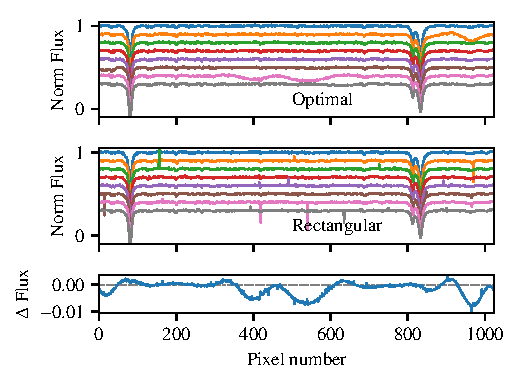
\includegraphics[width=0.7\linewidth]{figures/appendix/bp_plots/extraction_comparision_HD30501-2b_chip_2}
    \caption{Same as \fref{fig:artefact_example1} but for the second detector of the second observation of {HD\,30501}. In this example there are artefact causing spikes in four places. The second nod (orange) around pixel 950, the sixth nod (brown) around pixel 20 and two spikes in the seventh nod (pink) around pixels 400 and 550.}
    \label{fig:artefact_example7}
\end{figure}
